\begin{appendices}

\chapter{Tabellen}

\begin{table}[h]
	\centering

	\resizebox{\columnwidth}{!}{%
		\begin{tabular}{cccccccc}
			\hline 
			\multicolumn{1}{c}{} & \multicolumn{7}{c}{Barkley}\\ 
			\hline
			\rule[-1ex]{0pt}{2.5ex} $a$ & 4 & 8 & 16 & 32 & 64 & 128 & 148\\ 
			\rule[-1ex]{0pt}{2.5ex} $b$ & 2 & 2 & 2 & 2 & 1 & 2 & 1 \\ 
			\rule[-1ex]{0pt}{3.5ex} $N$ & 400 & 400 & 400 & 200 & 400 & 200 & 50\\ 
			\rule[-1ex]{0pt}{3.5ex} $\rho(|\mathbf{W}|)$ & 0.5 & 0.1 & 1.1 & 1.5 & 1.1 & 1.1 & 1.5\\ 
			\rule[-1ex]{0pt}{3.5ex} $\alpha$ & 0.95 & 0.95 & 0.20 & 0.05 & 0.05 & 0.20 & 0.05 \\ 
			\rule[-1ex]{0pt}{3.5ex} $\epsilon$ & 0.2 & 0.2 & 0.1 & 0.1 & 0.2 & 0.2 & 0.2 \\ 
			\rule[-1ex]{0pt}{3.5ex} $\nu_{max}$ & $\num{1e-4}$ & $\num{1e-4}$ & $\num{1e-5}$ & $\num{1e-4}$ & $\num{1e-5}$ & $\num{1e-4}$ &  $\num{1e-5}$\\ 
			\rule[-1ex]{0pt}{3.5ex} $\lambda$ & $\num{5e-4}$ & $\num{5e-4}$ & $\num{5e-0}$ & $\num{5e+2}$ & $\num{5e+4}$ & $\num{5e+3}$ & $\num{5e-0}$\\ 	
			\rule[-1ex]{0pt}{3.5ex} $\eta$ & 20 & 5 & 5 & 100 & 100 & 20 & 10\\		
			\\
			\rule[-1ex]{0pt}{2.5ex} Laufzeit [s] & 5 & 15 & 60 & 170 & 1922 & 3320 & 2970\\
			\rule[-1ex]{0pt}{2.5ex} \textbf{MSE} & \textbf{0.00005} & \textbf{0.00111} & \textbf{0.01447} & \textbf{0.09301} & \textbf{0.13093} & \textbf{0.15106} & \textbf{0.18380}\\ 
			\rule[-1ex]{0pt}{2.5ex} \textbf{NRMSE} & \textbf{0.0121} & \textbf{0.0801} & \textbf{0.3386} & \textbf{0.7398} & \textbf{0.9438} & \textbf{1.0098} & \textbf{1.1049} \\ 
			\hline 
		\end{tabular} 
		}
		\caption{Vollständige Auflistung der gefundenen Hyperparameter der \textsc{ESN}s für das \textit{Barkley}-Modell für verschiedene Größen $a$ des vorherzusagenden Bereichs, welche zu den geringsten Fehlern führen. Zudem sind die benötigte Laufzeit und die erreichten Fehler angeführt. Die Größe $b$ ist ebenfalls optimiert worden.}
\label{tab:apx_inner_cross_esn_results_barkley}
\end{table}

\begin{table}[t]
	\resizebox{\columnwidth}{!}{%
		\begin{tabular}{cccccccc}
		 	\hline 
			\multicolumn{1}{c}{} & \multicolumn{7}{c}{Mitchell-Schaeffer}\\ 
			\hline
			\rule[-1ex]{0pt}{2.5ex} $a$ & 4 & 8 & 16 & 32 & 64 & 128 & 148\\ 
			\rule[-1ex]{0pt}{2.5ex} $b$ & 1 & 3 & 2 & 2 & 1 & 2 & 1 \\ 
			\rule[-1ex]{0pt}{3.5ex} $N$ & 400 & 200 & 50 & 50 & 50 & 200 & 50\\ 
			\rule[-1ex]{0pt}{3.5ex} $\rho(|\mathbf{W}|)$ & 1.5 & 0.1 & 1.5 & 1.1 & 3.0 & 1.1 & 1.5\\ 
			\rule[-1ex]{0pt}{3.5ex} $\alpha$ & 0.95 & 0.95 & 0.50 & 0.20 & 0.50 & 0.20 & 0.70 \\ 
			\rule[-1ex]{0pt}{3.5ex} $\epsilon$ & 0.1 & 0.2 & 0.1 & 0.1 & 0.1 & 0.2 & 0.2 \\ 
			\rule[-1ex]{0pt}{3.5ex} $\nu_{max}$ & $\num{1e-4}$ & $\num{1e-4}$ & $\num{1e-4}$ & $\num{1e-4}$ & $\num{1e-5}$ & $\num{1e-4}$ &  $\num{1e-5}$\\ 
			\rule[-1ex]{0pt}{3.5ex} $\lambda$ & $\num{5e-0}$ & $\num{5e-1}$ & $\num{5e-0}$ & $\num{5e+3}$ & $\num{5e+3}$ & $\num{5e+4}$ & $\num{5e+4}$\\ 
			\rule[-1ex]{0pt}{3.5ex} $\eta$ & 20 & 50 & 15 & 5 & 100 & 10 & 15\\	
			\\ 			
			\rule[-1ex]{0pt}{2.5ex} Laufzeit [s] & 3 & 9 & 27 & 121 & 548 & 3322 & 3021\\
			\rule[-1ex]{0pt}{2.5ex} \textbf{MSE} & \textbf{0.00023} & \textbf{0.00177} & \textbf{0.02969} & \textbf{0.05061} & \textbf{0.06330} & \textbf{0.06842} & \textbf{0.06761}\\ 
			\rule[-1ex]{0pt}{2.5ex} \textbf{NRMSE} & \textbf{0.0661} & \textbf{0.1704} & \textbf{0.6703} & \textbf{0.8861} & \textbf{0.9775} & \textbf{1.0166} & \textbf{1.0049} \\ 
			\hline 
		\end{tabular} 
	}

	\caption{Vollständige Auflistung der gefundenen Hyperparameter der \textsc{ESN}s für das \textit{Mitchell-Schaeffer}-Modell (unten) für verschiedene Größen $a$ des vorherzusagenden Bereichs, welche zu den geringsten Fehlern führen. Zudem sind die benötigte Laufzeit und die erreichten Fehler angeführt. Die Größe $b$ ist ebenfalls optimiert worden.}
\label{tab:apx_inner_cross_esn_results_ms}
\end{table}


\chapter{Abbildungen}

\begin{figure}[h]
	\centering
	\begin{subfigure}{.5\textwidth}
		\centering
		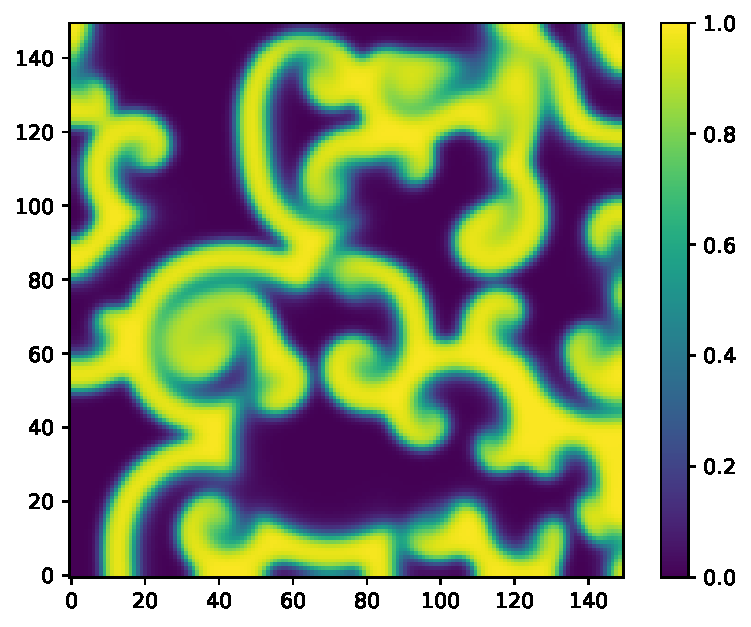
\includegraphics[height=2.5in]{figures/results/dynamics/barkley_0.pdf}
		\setcapmargin[1cm]{0.5cm}
		\caption{Erregung für $n=0$}
	\end{subfigure}%
	\begin{subfigure}{.5\textwidth}
		\centering
		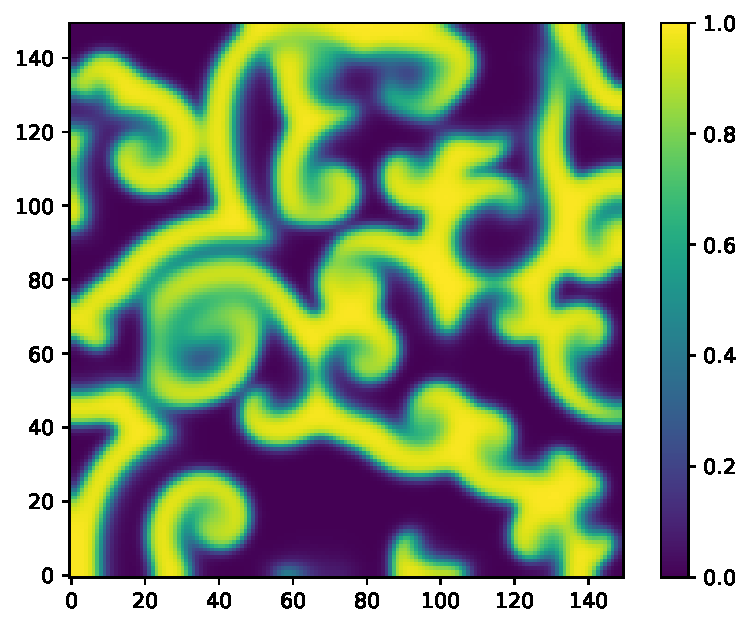
\includegraphics[height=2.5in]{figures/results/dynamics/barkley_50.pdf}
		\setcapmargin[1cm]{0.5cm}
		\caption{Erregung für $n=50$}
	\end{subfigure}
	\begin{subfigure}{.5\textwidth}
		\centering
		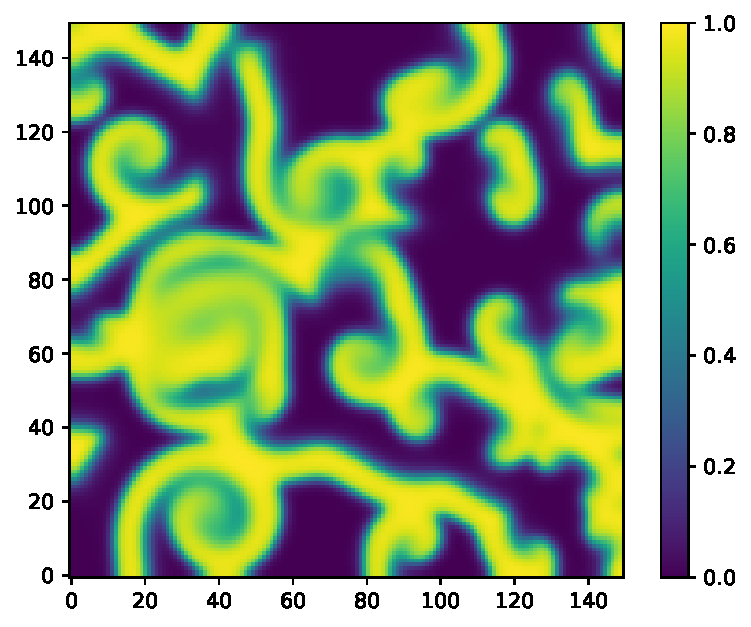
\includegraphics[height=2.5in]{figures/results/dynamics/barkley_100.pdf}
		\setcapmargin[1cm]{0.5cm}
		\caption{Erregung für $n=100$}
	\end{subfigure}%
	\begin{subfigure}{.5\textwidth}
		\centering
		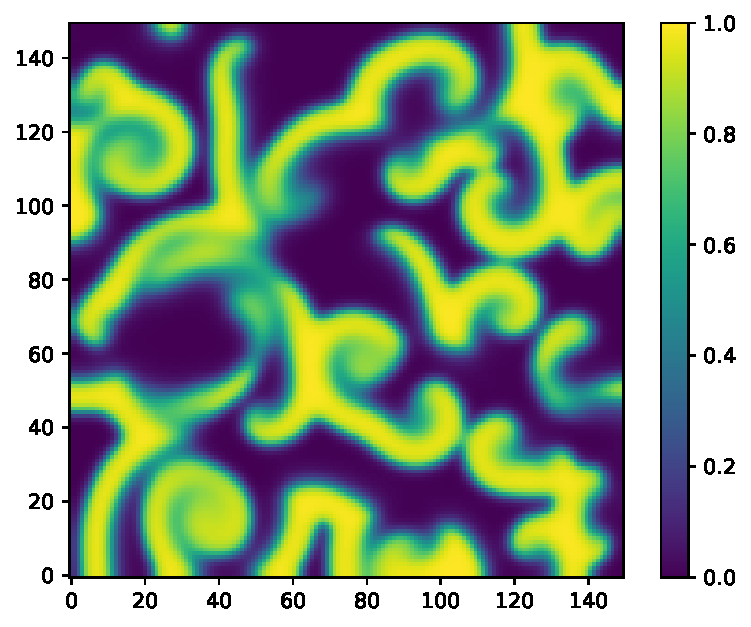
\includegraphics[height=2.5in]{figures/results/dynamics/barkley_150.pdf}
		\setcapmargin[1cm]{0.5cm}
		\caption{Erregung für $n=150$}
	\end{subfigure}
	\caption{Graphische Darstellung der zeitlichen Entwicklung der $u$-Variable des \textit{Barkley}-Modells. In Leserichtung sind die Felder der $u$-Variable für die Zeitpunkte $t=0,\, 50,\, 100,\, 150$ des Evaluationsdatensatzes dargestellt.}
	\label{fig:apx_barkley_evolution}
\end{figure} 

\begin{figure}[h]
	\centering
	\begin{subfigure}{.5\textwidth}
		\centering
		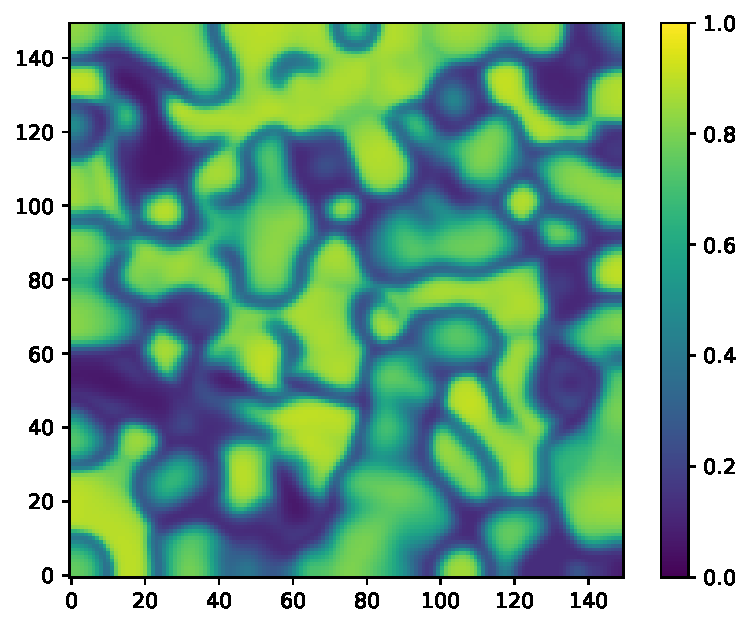
\includegraphics[height=2.5in]{figures/results/dynamics/mitchell_0.pdf}
		\setcapmargin[1cm]{0.5cm}
		\caption{Erregung für $n=0$}
	\end{subfigure}%
	\begin{subfigure}{.5\textwidth}
		\centering
		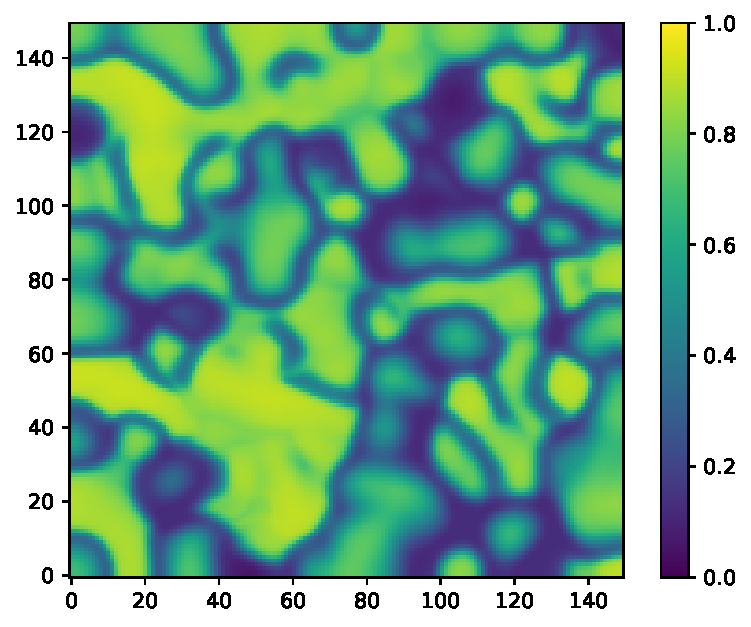
\includegraphics[height=2.5in]{figures/results/dynamics/mitchell_50.pdf}
		\setcapmargin[1cm]{0.5cm}
		\caption{Erregung für $n=50$}
	\end{subfigure}
	\begin{subfigure}{.5\textwidth}
		\centering
		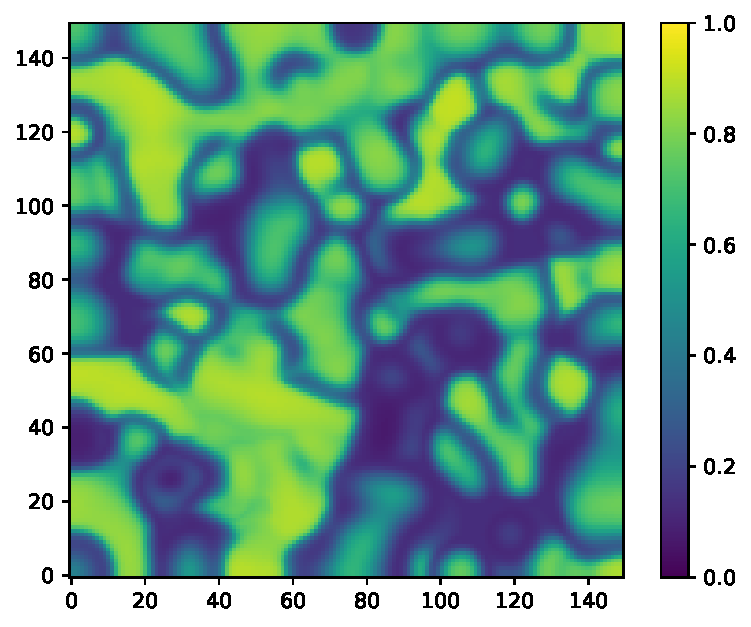
\includegraphics[height=2.5in]{figures/results/dynamics/mitchell_100.pdf}
		\setcapmargin[1cm]{0.5cm}
		\caption{Erregung für $n=100$}
	\end{subfigure}%
	\begin{subfigure}{.5\textwidth}
		\centering
		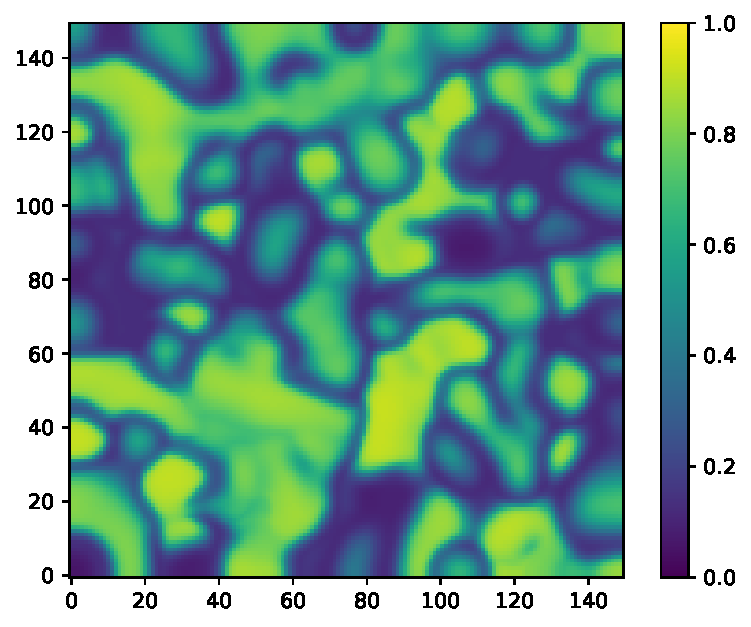
\includegraphics[height=2.5in]{figures/results/dynamics/mitchell_150.pdf}
		\setcapmargin[1cm]{0.5cm}
		\caption{Erregung für $n=150$}
	\end{subfigure}
	\caption{Graphische Darstellung der zeitlichen Entwicklung der $u$-Variable des \textit{Mitchell-Schaeffer}-Modells. In Leserichtung sind die Felder der $v$-Variable für die Zeitpunkte $n=0,\, 50,\, 100,\, 150$ des Evaluationsdatensatzes dargestellt.}
	\label{fig:apx_mitchell_evolution}
\end{figure} 

\begin{figure}[h]
	\centering
	\begin{subfigure}{.5\textwidth}
		\centering
		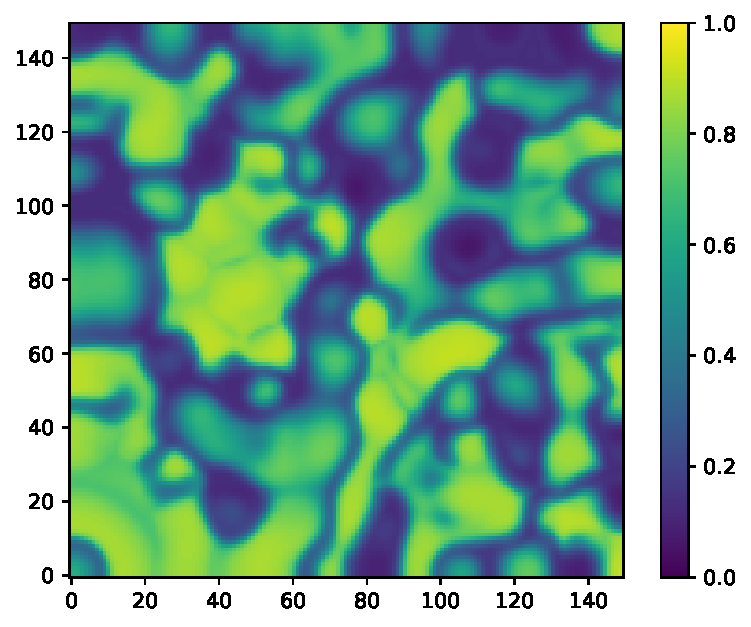
\includegraphics[height=2.5in]{figures/results/inner_cross_prediction/mitchell_v_inner_original.pdf}
		\setcapmargin[1cm]{0.5cm}
		\caption{Echte Erregung des Modells}
	\end{subfigure}%
	\begin{subfigure}{.5\textwidth}
		\centering
		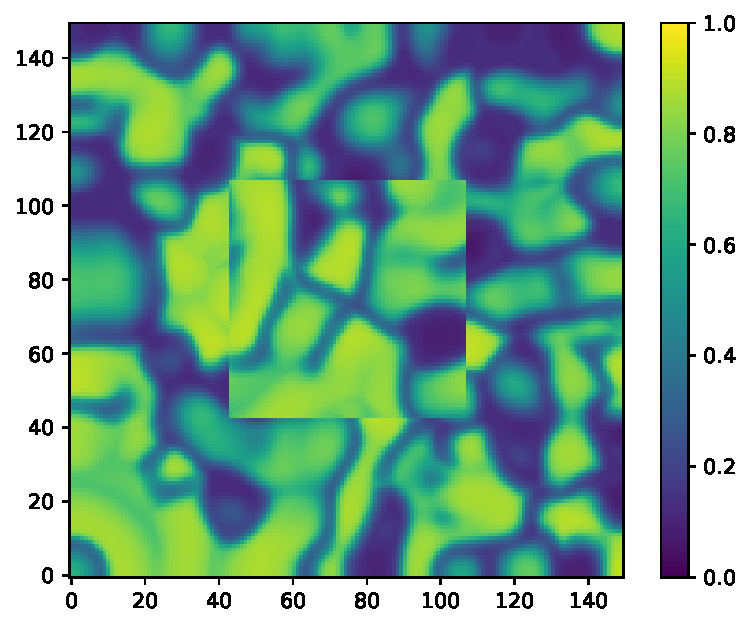
\includegraphics[height=2.5in]{figures/results/inner_cross_prediction/mitchell_v_inner_nn.pdf}
		\setcapmargin[1cm]{0.5cm}
  		\caption{Vorhersage des \textsc{NN}-Ansatzes}
	\end{subfigure}
	\begin{subfigure}{.5\textwidth}
		\centering
		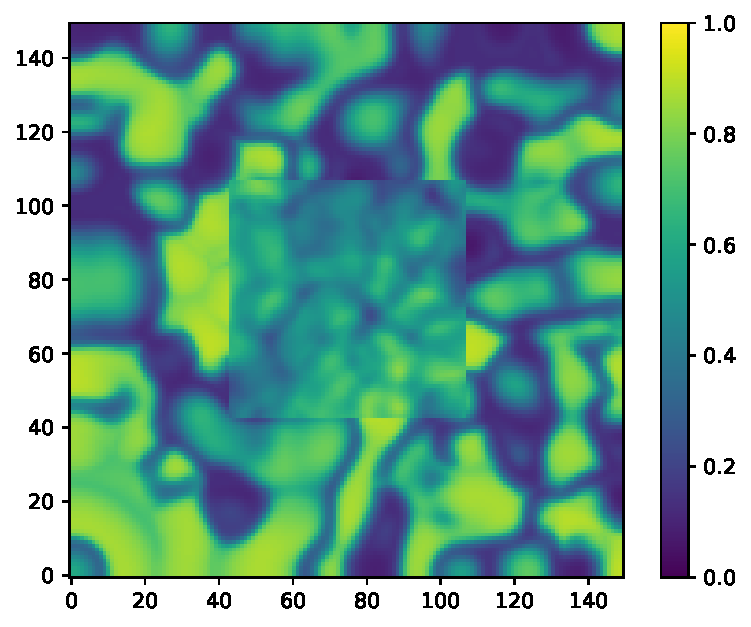
\includegraphics[height=2.5in]{figures/results/inner_cross_prediction/mitchell_v_inner_rbf.pdf}
		\setcapmargin[1cm]{0.5cm}
  		\caption{Vorhersage des \textsc{RBF}-Ansatzes}
	\end{subfigure}%
	\begin{subfigure}{.5\textwidth}
		\centering
		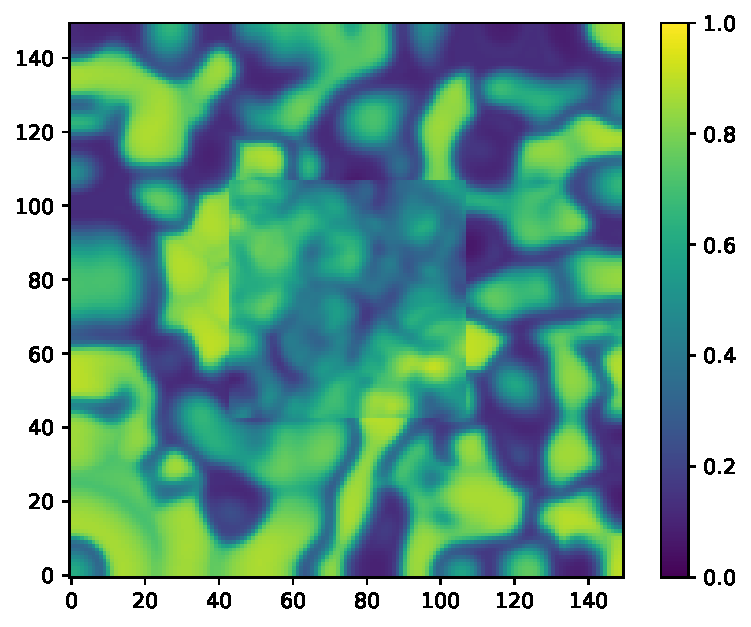
\includegraphics[height=2.5in]{figures/results/inner_cross_prediction/mitchell_v_inner_esn.pdf}
		\setcapmargin[1cm]{0.5cm}
  		\caption{Vorhersage des \textsc{ESN}}
	\end{subfigure}
	\caption{Graphische Darstellung der $v$-Variable des \textit{Mitchell-Schaeffer}-Modells für den $1000$. Zeitschritt des Evaluationsdatensatzes. Oben links ist das tatsächliche Feld des Modells zu sehen. Danach folgenden in Leserichtung die Vorhersagen des \textsc{NN}-Ansatzes, des \textsc{RBF}-Ansatzes und des \textsc{ESN}.}
	\label{fig:apx_inner_cross_mitchell_result}
\end{figure} 

\begin{figure}[h]
	\centering
	\begin{subfigure}{.95\textwidth}
		\centering
		\hspace*{0.18cm}
		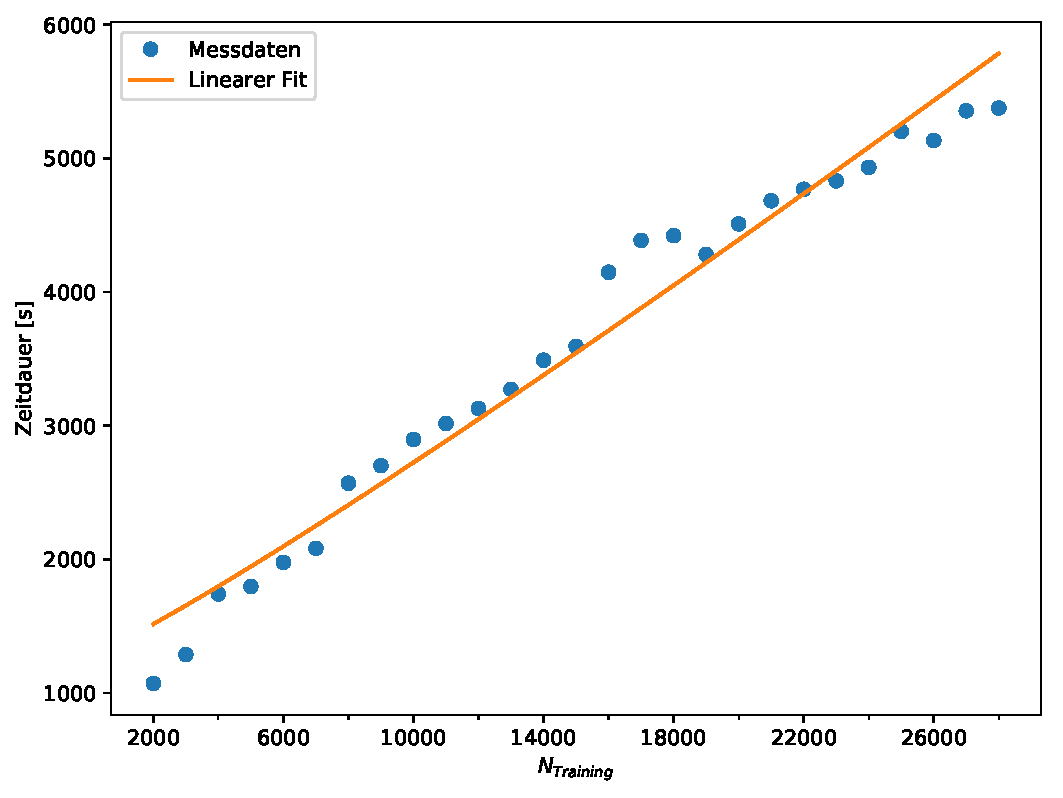
\includegraphics[width=4.8in]{figures/results/cross_prediction/nn_trainlength_vh_time.pdf}
		\caption{Abhängigkeit der Laufzeit.}
	\end{subfigure}
	\\
	\begin{subfigure}{.95\textwidth}
		\centering
		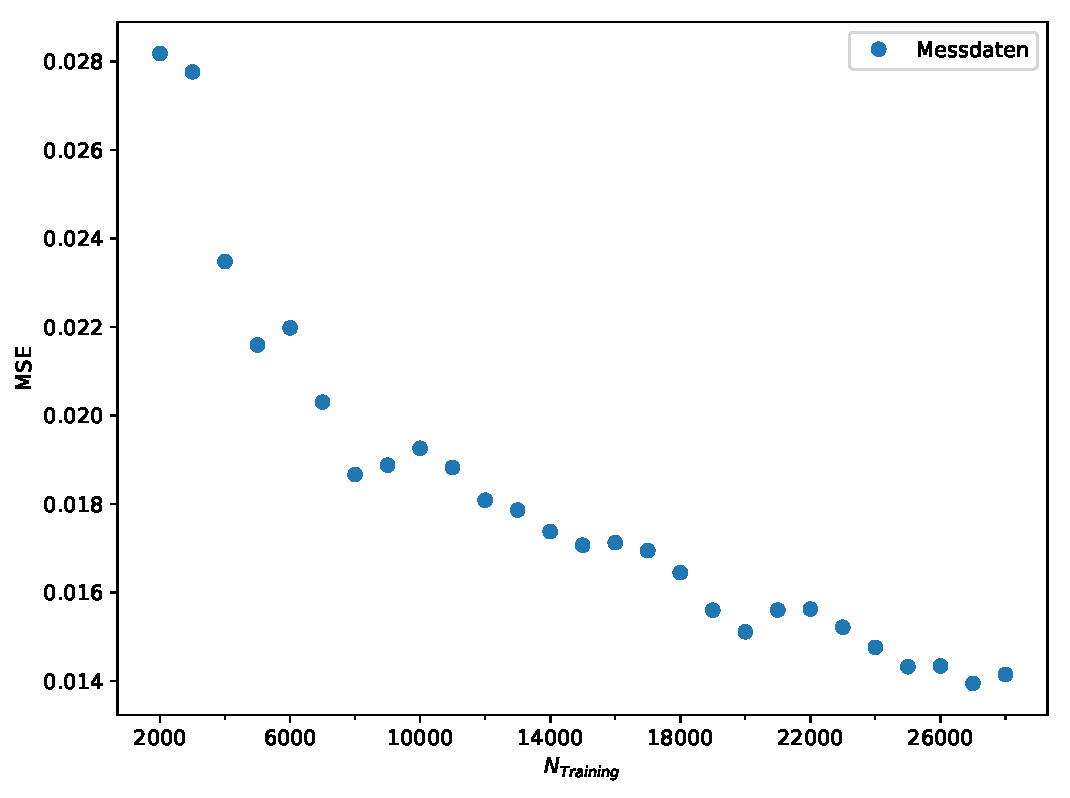
\includegraphics[width=4.8in]{figures/results/cross_prediction/nn_trainlength_vh_mse.pdf}
		\caption{Abhängigkeit des \textit{MSE}s.}
	\end{subfigure}
	\caption{Darstellung der Abhängigkeit des benötigten Laufzeit (oben) und des MSE (unten) von der verwendeten Anzahl an Trainingsdaten $N_{Training}$ (unten) für das \textit{Mitchell-Schaeffer}-Modell bei der Verwendung einer nächsten Nachbar Vorhersage.}
	\label{fig:apx_exp_cross_nn_trainlength_mse_time_ms}
\end{figure}


\begin{figure}[h]
	\centering
	\begin{subfigure}{\textwidth}
		\centering
		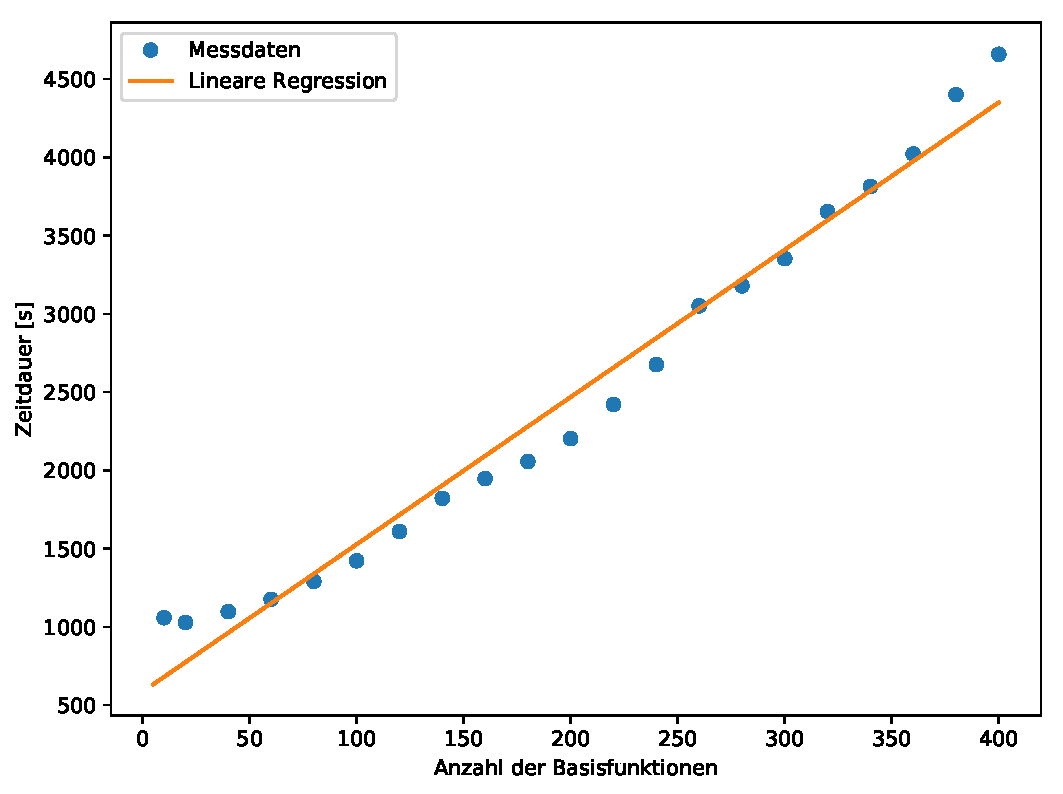
\includegraphics[width=4.8in]{figures/results/cross_prediction/rbf_placements_vh_time.pdf}
		\caption{Abhängigkeit der Laufzeit von $l$.}
	\end{subfigure}
	\begin{subfigure}{\textwidth}
		\centering
		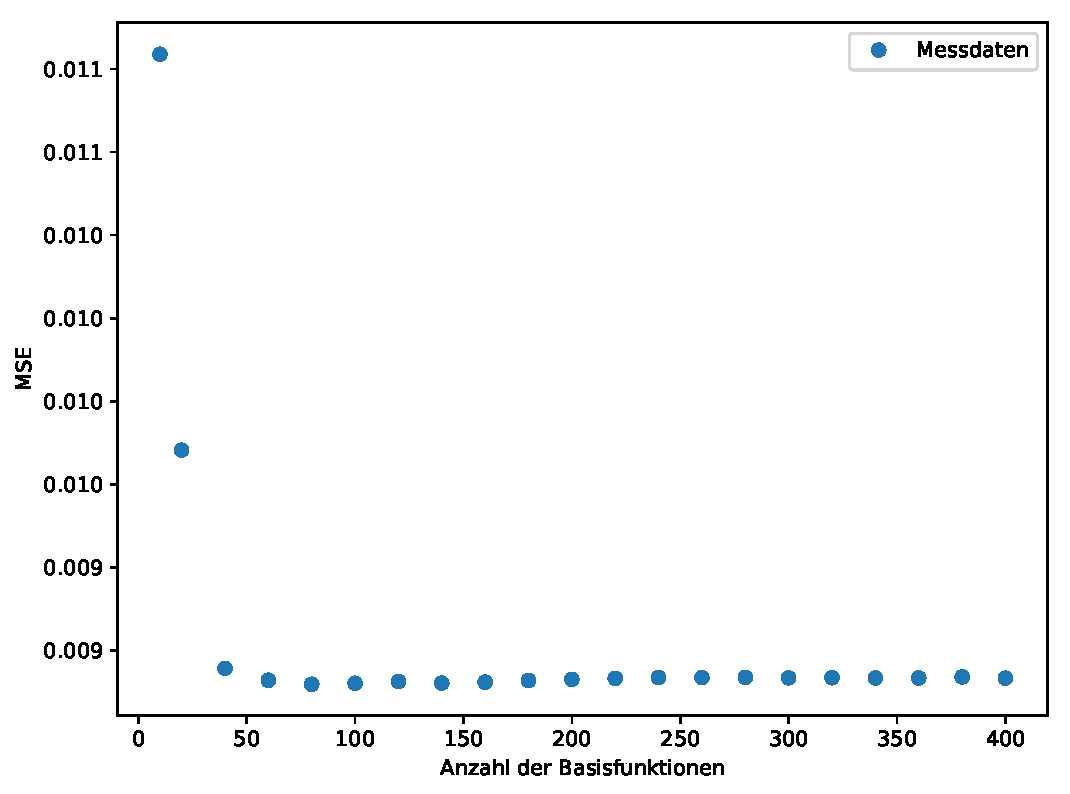
\includegraphics[width=4.8in]{figures/results/cross_prediction/rbf_placements_vh_mse.pdf}
  		\caption{Abhängigkeit des \textit{MSE}s von $l$.}
	\end{subfigure}
	\caption{Darstellung der Abhängigkeit des benötigten Laufzeit (oben) und des \textit{MSE}s (unten) von der Anzahl der Basisfunktionen $l$ für das \textit{Mitchell-Schaeffer}-Modell bei der Verwendung radialer Basisfunktionen.}
	\label{fig:apx_exp_cross_rbf_placements_time_mse_ms}
\end{figure}

\begin{figure}[h]
	\centering
	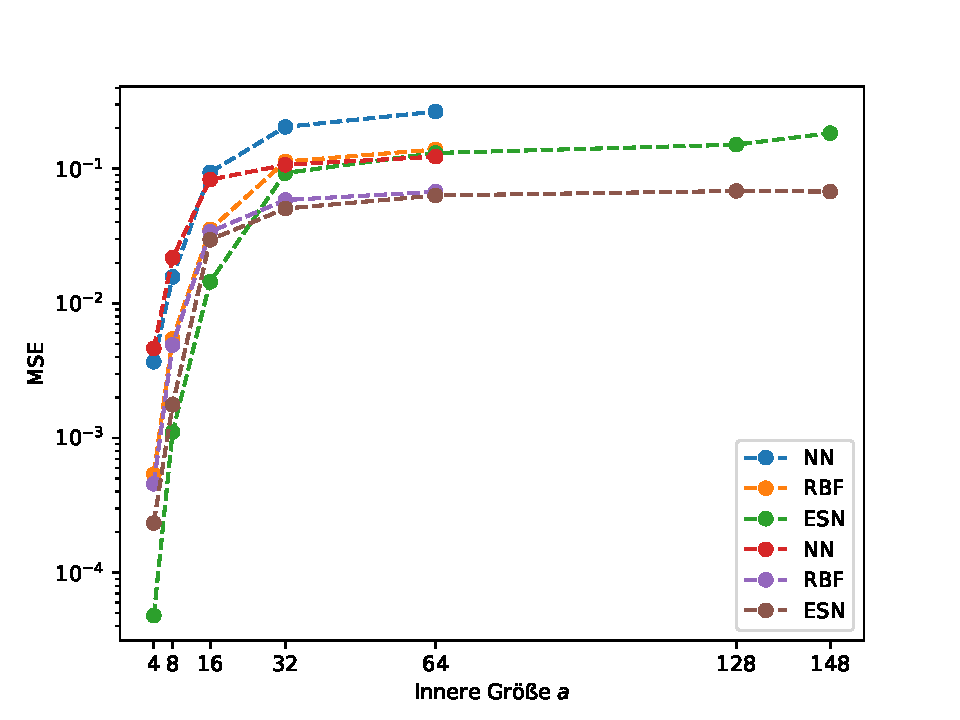
\includegraphics[height=4.2in]{figures/results/inner_cross_prediction/mitchell_error_size_comparison.pdf}
	\caption{Graphische Darstellung des Fehlerwertes MSE für die drei verschiedenen Ansätze in Abhängigkeit von der Größe $a$ des vorherzusagenden Bereichs für das \textit{Mitchell-Schaeffer}-Modell.}
	\label{fig:apx_inner_prediction_error_size_comparison_ms}
\end{figure} 


\chapter{Mathematische Ausführungen}
\section{Beweisskizze: Stabilitätskriterium}
\label{sc:apx_math_stability_proof}
Im Folgenden wird eine Beweisskizze für das Stabilitätskriterium
\begin{align*}
|1-\alpha(1-\sigma_{max}(\mathbf{W}))| < 1
\end{align*}
nach \cite{jaeger2010} vorgeführt. Hierfür wird die Distanz der \textit{l2-Norm} $||\cdot||$ zwischen den Zustandsfolgen $(\vec{s}(n))_n$ und $(\vec{s'}(n))_n$ für das Eingangssignal $\vec{u}$ betrachtet. Es wird zudem die Zustandsgleichung \ref{eq:esn_stateeq} und die Abkürzung $\vec{v} = [b_{in}; \vec{u}(n)]$ verwendet. 

\begin{align*}
&~||\vec{s}(n+1))- \vec{s}\,'(n+1)|| \\
&= ||(1 - \alpha) \cdot \vec{s}(n)  + \alpha \cdot f_{in}\left( \mathbf{W_{in}} \vec{v} + \mathbf{W} \vec{s}(n) \right) - (1 - \alpha) \cdot \vec{s}\,'(n)  - \alpha \cdot f_{in}\left( \mathbf{W_{in}} \vec{v} + \mathbf{W} \vec{s}\,'(n) \right)|| \\
&= || (1-\alpha)\cdot(\vec{s}(n)-\vec{s}\,'(n)) + \alpha \cdot f_{in}\left( \mathbf{W_{in}} \vec{v} + \mathbf{W} \vec{s}(n) \right) - \alpha \cdot f_{in}\left( \mathbf{W_{in}} \vec{v} + \mathbf{W} \vec{s}\,'(n) \right) ||\\
&\underset{\mathrm{(a)}}{\leq} (1-\alpha)\cdot|| \vec{s}(n)-\vec{s}\,'(n)|| + \alpha \cdot ||f_{in}\left( \mathbf{W_{in}} \vec{v} + \mathbf{W} \vec{s}(n) \right) - f_{in}\left( \mathbf{W_{in}} \vec{v} + \mathbf{W} \vec{s'}(n) \right) ||\\
&\underset{\mathrm{(b)}}{\leq} (1-\alpha)\cdot|| \vec{s}(n)-\vec{s}\,'(n)|| + \alpha \cdot ||\mathbf{W_{in}} \vec{v} + \mathbf{W} \vec{s}(n)- \mathbf{W_{in}} \vec{v} + \mathbf{W} \vec{s}\,'(n) ||\\
&= (1-\alpha)\cdot|| \vec{s}(n)-\vec{s}\,'(n)|| + \alpha \cdot ||\mathbf{W} \left(\vec{s}(n)- \vec{s}\,'(n) \right)||\\
&\underset{\mathrm{(c)}}{\leq} (1-\alpha)\cdot ||\vec{s}(n)-\vec{s'}(n)|| + \alpha \cdot \sigma_{max}\left(\mathbf{W}\right)||\vec{s}(n)- \vec{s}\,'(n) ||\\
&= \left(1-\alpha+\alpha\sigma_{max} \left(\mathbf{W} \right) \right) \cdot ||\vec{s}(n)-\vec{s}\,'(n)|| \\
&= \left(1-\alpha(1+\sigma_{max} \left(\mathbf{W} \right)) \right) \cdot ||\vec{s}(n)-\vec{s}\,'(n)|| \\
&:= \lambda ||\vec{s}(n)-\vec{s'}(n)||
\end{align*}

Dabei ist in Schritt $\mathrm{(a)}$ die Dreiecksungleichung verwendet worden. Da $f_{in}$ eine \textit{sigmoid}-förmige Funktion ist, gilt zudem $f'_{in}(x) < 1 \forall x$; dies wird in Schritt $\mathrm{(b)}$ ausgenutzt. Zudem wird in Schritt $\mathrm{(c)}$ die Beziehung
\begin{align*}
||\mathbf{A} \vec{x}|| \leq \sigma_{max}\left(\mathbf{A} \right) ||\vec{x}||
\end{align*}
zwischen dem maximalen Sprektralwert $\sigma_{max}$ der Matrix $\mathbf{A}$ und der \textit{l2-Norm} ausgenutzt.\\

Gilt nun $\lambda < 1$, so nähern sich die beiden Zustandsfolgen immer näher aneinander an, bis sie schließlich gegeneinander konvergieren. Das bedeutet, dass es eine Nullfolge $(\delta(n))_n$ gibt, für die $||\vec{s}(n) - \vec{s}\,'(n)|| < \delta(n)$; somit liegt die \textit{ESP} vor. Dies bedeutet, dass der beliebig gewählte Anfangszustand des \textsc{ESN}s $\vec{s}(0)$ beziehungsweise $\vec{s}\,'(0)$ nach einer ausreichenden Zeit keinen Einfluss mehr auf die Dynamik des Systems nimmt.

\section{Laufzeitanalyse}
\label{sc:apx_runtime_complexity}
Im Folgenden soll die theoretische Laufzeitkomplexität $T$ des Trainings und Vorhersagevorgangs eines \textsc{ESN}s unter Veränderung von $N$ betrachtet und hergeleitet werden.
Zuerst werden die Abkürzungen
\begin{align*}
\beta = T-T_{0} \qquad\qquad\qquad \gamma = 1+N_u+N
\end{align*}
eingeführt. Für die Matrixmultiplikation und Matrixinversion wird ein optimierter Algorithmus wie beispielsweise der \textit{Coppersmith–Winograd}-Algorithmus angenommen. Dieser hat für Matrizen $\in \mathbb{R}^{n \times n}$ eine Laufzeit $\mathcal{O}(n^{2.376})$. \improvement{Add source}\\
Die Komplexität der Zustandsgleichung \ref{eq:esn_stateeq} wird durch die Ausdrücke $\mathbf{W_{in}} \vec{u} \in \mathcal{O}(N_U N)$ und $\mathbf{W}\vec{x} \in \mathcal{O}(N^2)$ bestimmt. Somit ergibt sich eine Gesamtkomplexität $\mathcal{O}(N_u \cdot N + N^2) = \mathcal{O}(N^2)$ für $N_u < N$.\\

Im Trainingsvorgang wird zunächst die Zustandsgleichung $\beta$ Mal durchlaufen. Bei der Betrachtung der Lösungsgleichung \ref{eq:tikhonov} müssen die Laufzeiten von vier Teilausdrücken analysiert werden:
\begin{align*}
T\left(\mathbf{X}\mathbf{X}^T \right) = \mathcal{O}(\gamma^2 \beta) \\
T\left((\mathbf{X}\mathbf{X})^{-1} \right) = \mathcal{O}(\gamma^{2.376}) \\
T\left(\mathbf{Y_{target}}\mathbf{X}^T \right) = \mathcal{O}(N_y \beta \gamma).
\end{align*}
Somit ergibt sich für das Bestimmten der Auslesematrix $\mathbf{W_{out}}$ eine Laufzeit $\mathcal{O}(\gamma^2 \beta + \gamma^{2.376} + \beta \gamma N_y) = \mathcal{O}(\gamma^{2.376})$  für $N_u < N$.
Insgesamt ergibt sich der Aufwand des Trainingsvorgangs somit inklusive der Berechnung der Zustandsgleichung zu $\mathcal{O}(N^2 + N^{2.376}) = \mathcal{O}(N^{2.376})$\\

Der Vorhersagevorgang besteht jeweils aus Berechnungen der Zustandsgleichung und der  Berechnung der Ausgabe $\vec{y} = \mathbf{W_{out}} \vec{x}$. Hierbei ergibt sich analog die Laufzeitkomplexität zu $\mathcal{O}(N^2)$.\\

Bei dieser Betrachtung sind noch nicht die auftretenden Laufzeiten durch das Initialisieren der Matrizen im Speicher und das Berechnen des Spektralradius zur Reskalierung von $\mathbf{W}$ berücksichtigt. 

\chapter{Programmüberblick}

\begin{figure}[h]
	\centering
	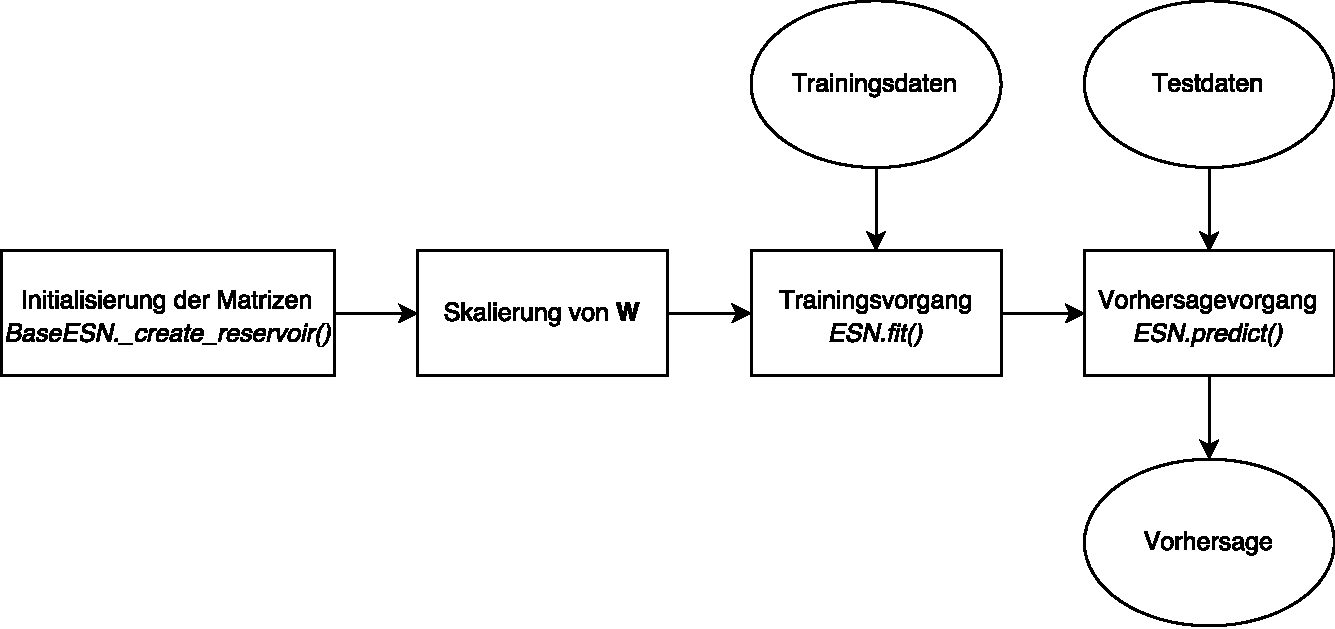
\includegraphics[width=0.9\textwidth]{figures/illustrations/esn_flow_chart.pdf}
  	\caption{Ablauf bei Verwendung eines \textsc{ESN}s. Dabei dabei relevanten Funktionen des Quellcodes sind kursiv geschrieben. In Leserichtung wird zuerst das \textsc{ESN} mit seinen Matrizen $\mathbf{W}$ und $\mathbf{W_{in}}$ generiert. Anschließend wird es trainiert (siehe Abbildung \ref{fig:apx_esn_training_flowchart}), um danach eine Vorhersage durchzuführen.}
  	  \label{fig:apx_esn_flowchart}
\end{figure}%

\begin{figure}[h]
	\centering
	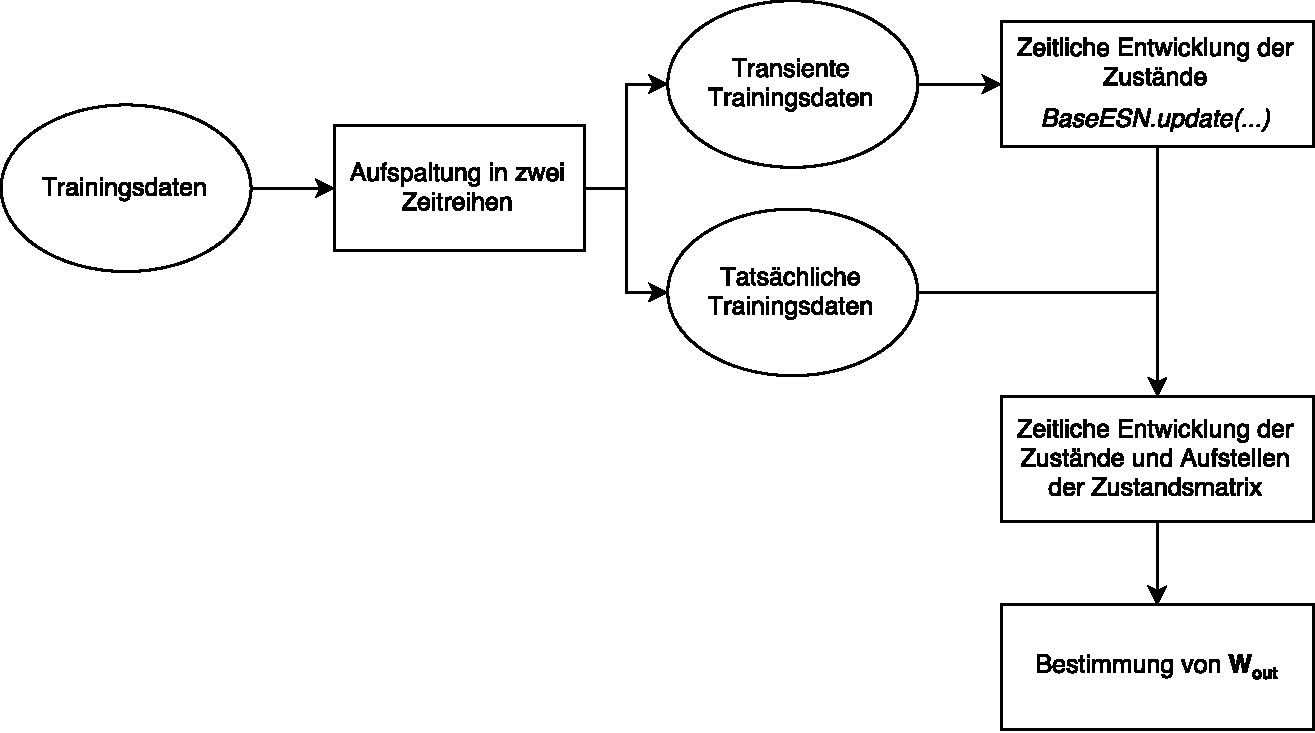
\includegraphics[width=0.9\textwidth]{figures/illustrations/esn_training_flow_chart.pdf}
  	\caption{Ablaufes des Trainingsvorgangs des \textsc{ESN}s. Zuerst wird die Zeitreihe der Trainingsdaten in zwei Zeitreihen unterteilt. Der erste Teil wird benutzt um das \textit{transiente} Verhalten des Reservoirs abzuwarten, wohingegen der Rest benutzt wird, um die Auslesematrix $\mathbf{W_{out}}$ zu bestimmen.}
  	\label{fig:apx_esn_training_flowchart}
\end{figure}%

\begin{figure}[h]
	\centering
	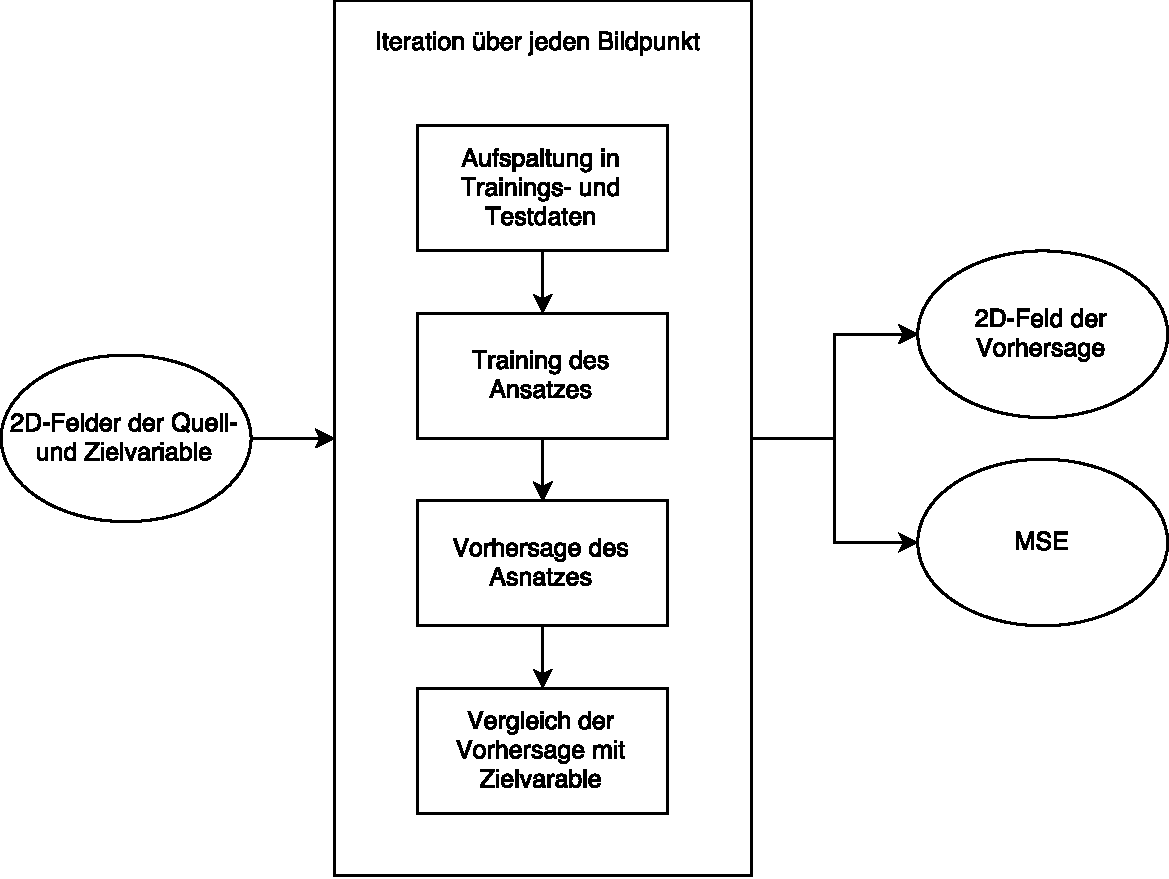
\includegraphics[width=0.9\textwidth]{figures/illustrations/general_predicition_flow_chart.pdf}
  	\caption{Allgemeines Vorgehen zum Bestimmen der Vorhersage in einem zweidimensionalen System. Für jeden Bildpunkt wird eine einzelne Zeitreihe betrachtet, welche in Trainings- und Testdaten unterteilt wird. Mit den Trainingsdaten wird nun das ausgewählte Modell (\textsc{NN}-Ansatz, \textsc{RBF}-Ansatz oder \textsc{ESN}) trainiert. Anschließend liefert das Modell mit der Quellvariable der Testdaten eine Vorhersage, welche mit den Zielvariable verglichen wird. Daraus kann der \textit{MSE} bestimmt werden. Durch das Durchführen dieser Prozedur für alle Bildpunkt ergibt sich schlussendlich eine Vorhersage des räumlich ausgedehnten Systems.}
  	  \label{fig:apx_general_prediction_flowchart}
\end{figure}%

\end{appendices}